\documentclass[a4,11pt]{article}
\usepackage{geometry}
\geometry{a4paper, top=40mm, left=30mm, right=30mm, bottom=40mm} % bottom und top 40

\usepackage{multicol}
\usepackage{color}

\setlength\parindent{0pt}
\usepackage[german]{babel}
\usepackage[utf8]{inputenc}

\usepackage{amsmath, amsthm, amssymb}
\usepackage{bm}
\usepackage{url}
\usepackage{physics}
\usepackage{enumitem}

\usepackage{caption}
\usepackage{graphicx, wrapfig}
\usepackage{subcaption} %z.B. in figure umgebungen um einzelne bilder zu benennen

\usepackage[version=4]{mhchem}
\usepackage{tikz}
%\usetikzlibrary{matrix}
%\usetikzlibrary{circuits.ee.IEC}
%%Volt- und Amperemeter festlegen:
%\tikzset{circuit declare symbol = ammeter}
%\tikzset{set ammeter graphic ={draw,generic circle IEC, minimum size=5mm,info=center:A}}
%\tikzset{circuit declare symbol = voltmeter}
%\tikzset{set voltmeter graphic ={draw,generic circle IEC, minimum size=5mm,info=center:V}}
\usepackage[european]{circuitikz}
\usetikzlibrary{arrows}
\newcommand{\mymeter}[2] 		% Option um Schaltsymbole zu drehen
{  % #1 = name , #2 = rotation angle
	\begin{scope}[transform shape,rotate=#2]
		\draw[thick] (#1)node(){$\mathbf V$} circle (11pt);
		\draw[rotate=45,-latex] (#1)  +(-17pt,0) --+(17pt,0);
	\end{scope}
}
\usepackage[
	disable,
	colorinlistoftodos,
	linecolor=yellow,
	backgroundcolor=yellow,
	textwidth=0.15\textwidth,
	textsize=footnotesize]{todonotes}

\usepackage[
locale=DE,
separate-uncertainty=true, % Immer Fehler mit ±
per-mode=symbol-or-fraction, % m/s im Text, sonst \frac
% alternativ:
% per-mode=reciprocal,
% m s^{-1}
output-decimal-marker=., % . statt , für Dezimalzahlen
]{siunitx}


\usepackage{fancyhdr}	%Kopf- und Fußzeile gestalten
\pagestyle{fancy}
\renewcommand{\sectionmark}[1]{\markright{#1}}
\renewcommand{\subsectionmark}[1]{\markright{#1}}
\fancyhead{}				%Default-Einstellungen im Header löschen
%\fancyhead[L]{\sc{Relaxationsverhalten eines RC-Kreises}}
\fancyhead[R]{\sc{\rightmark}}
% \leftmark sind die Sections \rightmark sind dei Subsections






\newcommand{\Versuch}{Das Michelson-Interferometer}
\newcommand{\Betreuer}{Julia \textsc{Mustermann}}
\newcommand{\Tag}{19.04.16}
\newcommand{\V}{V401}

% Bibliographie erstellen:
% 	pdflatex Protokoll.tex
% 	biber Protokoll
% 	pdflatex Protokoll.tex
% oder einfach make ausführen

\begin{document}
\begin{titlepage}
	\par
	\raisebox{-.5\height}{
\includegraphics[height=1cm]{../Vorlage/Logo-TUDo.png}}
	\hfill
	\raisebox{-.5\height}{
\includegraphics[height=1cm]{../Vorlage/Logo-Physik.png}}
	\par
\begin{center}
\ \\
[6cm]	
	\textsc{\Huge Anfängerpraktikum 2015/2016} \\
[2cm]
	\Huge\textbf{\Versuch} \\
[1cm]
	{\large Durchführung: \Tag} \\
[5cm]
\begin{minipage}{0.4\textwidth}
	\begin{flushleft} \large
		Clara \textsc{Rittmann}\textsuperscript{1} \\
		Anja \textsc{Beck}\textsuperscript{2}
	\end{flushleft}
\end{minipage}
\hfill
\begin{minipage}{0.4\textwidth}
	\begin{flushright} \large
		\emph{Betreuer:} \\
		\Betreuer
	\end{flushright}
\end{minipage}
\end{center}
\footnotetext[1]{clara.rittmann@tu-dortmund.de}
\footnotetext[2]{anja.beck@tu-dortmund.de}
\end{titlepage}


\tableofcontents
\clearpage


\section{Theorie}
Stoffe können in verschiedenen Aggregatszuständen auftreten. Diese hängen von der Temperatur und dem Druck ab. Sie werden auch Phasen genannt. Abbildung \ref{Phasendiagramm} zeigt ein schematisches Phasendiagramm von Wasser. Liegt beispielsweise flüssiges Wasser vor, dann können Temperatur und Druck innerhalb des Phasenraums (also ohne überschreiten einer Linie) beliebig variiert werden, ohne den Aggregatszustand zu ändern.
\begin{figure}[ht!]
	\centering
	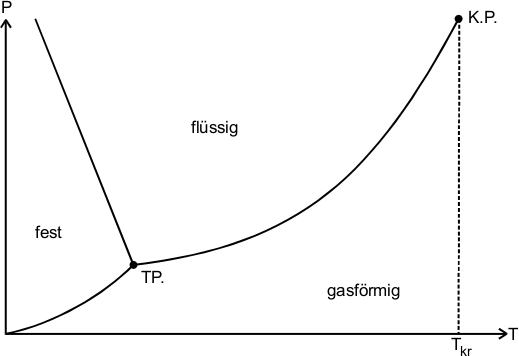
\includegraphics[width=0.9\textwidth]{Phasendiagramm.png}
	\caption{Phasendiagramm für Wasser\cite{V203}}
	\label{Phasendiagramm}
\end{figure} \\
Am Triple Punkt (TP) treten alle drei Phasen gleichzeitig auf. Die Kurve, die dort beginnt und die flüssige von der gasförmigen Phase trennt heißt Dampfdruckkurve. Hier hängen $p$ und $T$ voneinander ab. Diesen Zusammenhang beschreibt die Clausius-Clapeyronische Gleichung
\begin{equation}\label{Clausius}
	(V_\text{D}-V_\text{F})\ dp = \frac{L}{T}\ dT.
\end{equation}
Dabei ist $V_\text{D}$ das molare Volumen des Gases, $V_\text{F}$ das molare Volumen der Flüssigkeit, $T$ die Temperatur in Kelvin und $L$ die molare Verdampfungswärme. \\
Letztere ist die Menge Energie, die benötigt wird, um ein Mol Flüssigkeit bei konstanter Temperatur $T$ in Dampf umzuwandeln. $L$ ist abhängig vom Stoff und der Temperatur. In der Nähe des kritischen Punktes (siehe Abblidung \ref{Phasendiagramm}) verschwindet $L$, da es keinen Unterschied mehr zwischen flüssiger und gasförmiger Phase gibt. \\
Ist die Temperatur allerdings weit unter der kritischen Temperatur \[T_\text{Kr, Wasser} = \SI{374}{\celsius},\] kann $L$ als konstant betrachtet werden. Außerdem kann angenommen werden, dass $V_\text{F}$ vernachlässigbar gegenüber $V_\text{D}$ ist und $V_\text{D}$ der idealen Gasgleichung
\begin{equation}\label{ideales Gas}
	V_\text{D} = R\frac{T}{p}
\end{equation}
gehorcht. Dann vereinfacht sich die Clausius-Clapeyronische Gleichung zu
\begin{equation}\label{Clausius einfach}
	\frac{1}{p}\ dp = \frac{1}{R}\frac{L}{T^2}\ dT
\end{equation}
bzw. nach Integration
\begin{equation}\label{Regression ln(p)=1/T}
	\ln p = - \frac{1}{R}\frac{L}{T} + \frac{L}{RT_0}+\ln p_0.
\end{equation}
\clearpage


\section{Versuchsaufbau: Das Michelson-Interferometer}
Ziel des Versuches ist es, den Brechungsindex und die Dispersionskurve eines Gases zu bestimmen.
Dies geschieht mit Hilfe eines Prismas, einer Cadmium-Quecksilber-Lampe, eines Fernsrohs und eines Winkelmessers, die wie in Abbildung~\ref{fig:aufbau} gezeigt angeordnet sind. Die Lampe ist fest. Vor ihr ist auf einer drehbaren Platte mit Winkelanzeige das Prisma angebracht. Ein Fernrohr ist darum herum schwenkbar. \\

\begin{figure}[h!]
	\centering
	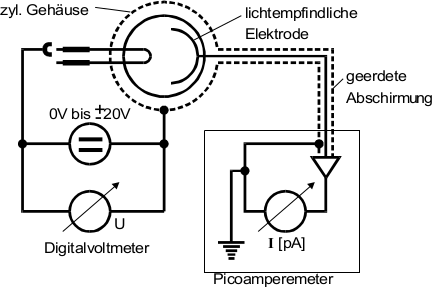
\includegraphics[width=0.8\textwidth]{Aufbau.png}
	\caption{Versuchsaufbau \cite{V402}}
	\label{fig:aufbau}
\end{figure}

An dem Prisma wird der Lichtstrahl doppelt gebrochen. Zur Berechnung des Brechungsindex ist zum einen der Winkel  $\eta$ zwischen eingehendem und ausgehendem Stahl relevant zum anderen der Innenwinkel $\varphi$ des Prismas. Wobei hier ein gleichseitiges Prisma vorliegt. Mit Hilfe des Snelliusschen Gesetz \eqref{eq:snellius}, das auf eine Doppelbrechung, wie in Abbildung~\ref{fig:prisma1} dargestellt, angewendet wird, folgt der Brechungsindex
\begin{align}\label{BrechIndex}
	n=\frac{\sin\frac{\eta + \varphi}{2}}{\sin\frac{\varphi}{2}} \quad .
\end{align}

\begin{figure}[h!]
	\centering
	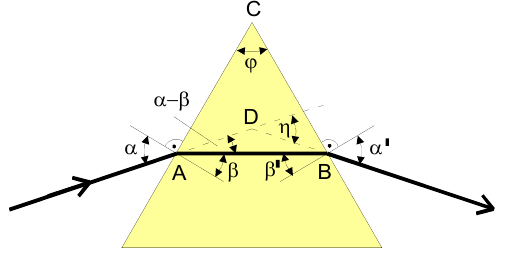
\includegraphics[width=0.7\textwidth]{Prisma1.png}
	\caption{Doppelbrechung am Prisma \cite{V402}}
	\label{fig:prisma1}
\end{figure}

\clearpage

\subsection{Messung des Innenwinkels $\varphi$}
Zur Messung des Innenwinkels $\varphi$ wird das Prisma so ausgerichtet, dass eine Spitze auf die Lampe zeigt und dann unverändert in dieser Position gelassen. Durch das Fernglas wird eine Spektrallinie der Lampe, die auf der Prismenoberfläche zu sehen ist erst auf der einen Seite des Prismas, dann auf der anderen Seite anvisiert. Jeweils wird der Winkel $\varphi_r$ bzw. $\varphi_l$ notiert. Aus Abbildung \ref{fig:prisma2} folgt mit einfacher Geometrie
\begin{align}\label{Phi}
	\varphi = \frac{1}{2} (\varphi_r - \varphi_l) \quad.
\end{align}

\begin{figure}[h!]
	\centering
	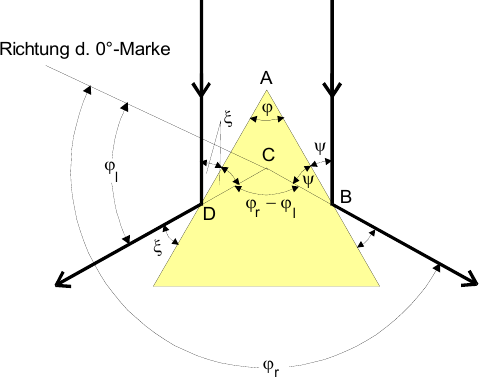
\includegraphics[width=0.42\textwidth]{Prisma2.png}
	\caption{Innenwinkelmessung \cite{V402}}
	\label{fig:prisma2}
\end{figure}

\subsection{Messung des Brechungswinkels $\eta$}
Im Gegensatz zur Messung des Innenwinkels wird bei der Bestimmung des Brechungswinkels das Prisma rotiert und das Fernrohr an einem festen Ort gelassen. \\
Fernrohr und Prisma werden einmalig so ausgerichtet, das die Spektrallinien zu sehen sind. Eine Linie wird ausgewählt und beobachtet. Dann wird das Prisma so lange gedreht, bis dieselbe Spektrallinie wieder im Fadenkreuz des Fernrohres liegt. Die Winkel beider Einstellungen $\Omega_r$ und $\Omega_l$ dienen zur Berechnung der Brechungswinkels $\eta$
\begin{align}\label{Eta}
	\eta = 180 - (\Omega_l - \Omega_r) \quad .
\end{align}
Der Vorgang ist in Abbildung \ref{fig:prisma3} dargestellt.

\begin{figure}[h!]
	\centering
	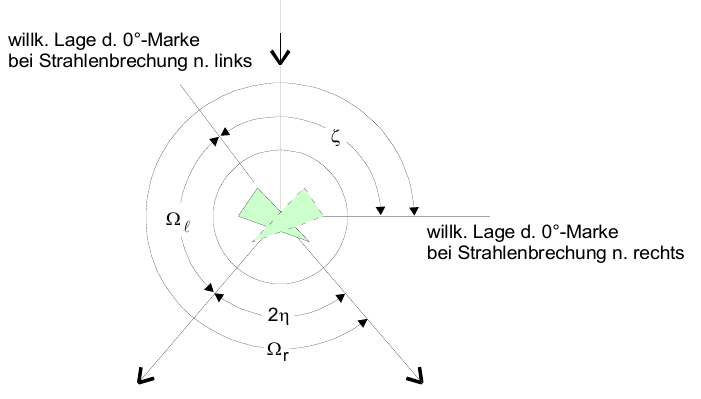
\includegraphics[width=0.57\textwidth]{Prisma3.png}
	\caption{Brechungswinkelmessung \cite{V402}}
	\label{fig:prisma3}
\end{figure}


\clearpage


\section{Auswertung}
%\subsection{Statistische Formeln}
%\subsubsection{Fehlerrechnung}
%\label{sec:Fehlerrechnung}
%<<<<<<< HEAD
Im folgenden wurden Mittelwerte von N Messungen der Größe $x$ berechnet
\begin {equation}
\bar{x} =  \frac{1}{N} \sum_{i=1}^\text{N} x_i
\end{equation}

sowie die Varianz
\begin {equation}
V(x) = \frac{1}{N-1} \sum_{i=1}^\text{N} (x_i - \bar{x})^2
\end{equation}

woraus die Standartabweichung folgt
\begin {equation}
\sigma_x = \sqrt{V(x)}.
\end{equation}

Die Standartabweichung des Mittelwertes, kürzer auch Fehler des Mittelwertes genannt, bezieht noch die Anzahl der Messungen mit ein. Mehr Messungen führen zu einem kleineren Fehler
\begin {equation}
\Delta_{x} = \frac{\sigma_x}{\sqrt{N}}.
\end{equation}
Im folgenden wurden Mittelwerte von N Messungen der Größe $x$ berechnet
\begin {equation}
\bar{x} =  \frac{1}{N} \sum_{i=1}^\text{N} x_i
\end{equation}

sowie die Varianz
\begin {equation}
V(x) = \frac{1}{N-1} \sum_{i=1}^\text{N} (x_i - \bar{x})^2
\end{equation}

woraus die Standartabweichung folgt
\begin {equation}
\sigma_x = \sqrt{V(x)}.
\end{equation}

Die Standartabweichung des Mittelwertes, kürzer auch Fehler des Mittelwertes genannt, bezieht noch die Anzahl der Messungen mit ein. Mehr Messungen führen zu einem kleineren Fehler
\begin {equation}
\Delta_{x} = \frac{\sigma_x}{\sqrt{N}}.
\end{equation}

%\subsubsection{Regression}
%\label{sec:regression}
%Nachfolgend wird eine lineare Regression für Wertepaare $(x_i,y_i)$ durchgeführt. Dafür müssen die Steigung
\begin{equation}
	m = \dfrac{
		n\cdot\sum\limits_{i=1}^nx_iy_i-\sum\limits_{i=1}^nx_i\cdot\sum\limits_{i=1}^ny_i
		}
		{n\cdot\sum\limits_{i=1}^nx_i^2-\left(\sum\limits_{i=1}^nx_i\right)^2
		}
\end{equation}
und der y-Achsenabschnitt
\begin{equation}
	b = \dfrac{
		\sum\limits_{i=1}^nx_i^2\cdot\sum\limits_{i=1}^ny_i-\sum\limits_{i=1}^nx_i\cdot\sum\limits_{i=1}^nx_iy_i
		}{
		n\cdot\sum\limits_{i=1}^nx_i^2-\left(\sum\limits_{i=1}^nx_i\right)^2
		}
\end{equation}
berechnet werden. Den jeweiligen Fehler erhält man mit
\begin{equation}
	s_m^2 = s_y^2 \cdot \dfrac{n}{n\cdot\sum\limits_{i=1}^nx_i^2-\left(\sum\limits_{i=1}^nx_i\right)^2}
\end{equation}
\begin{equation}
	s_b^2 = s_y^2 \cdot \dfrac{\sum\limits_{i=1}^nx_i^2}{n\cdot\sum\limits_{i=1}^nx_i^2-\left(\sum\limits_{i=1}^nx_i\right)^2}\ .
\end{equation}
$s_y$ ist hierbei die Abweichung der Regressionsgeraden in y-Richtung.
\begin{equation}
	s_y^2 = \dfrac{\sum\limits_{i=1}^n\left(\Delta y_i\right)^2}{n-2} = \dfrac{\sum\limits_{i=1}^n\left(y_i-b-mx_i\right)^2}{n-2}
\end{equation}
%\clearpage
\subsection{Fouriersynthese}
\begin{figure}[h!]
	\centering
	\captionof{table}{Fourier-Koeffizienten}
	\begin{tabular}{c|ccc}
		& Dreieck & Rechteck & Sägezahn \\
		\hline
		k=1 & 628.84    & 631.02  & -627.10  \\
		k=2 & 0    & 0  & -313.60  \\
		k= 3 & 69.87  & 210.34  & -209.03  \\
		k= 4 & 0  & 0  & -156.78  \\
		k=5 & 25.15  & 126.20  & -125.42   \\
		k= 6 & 0  & 0  & -104.52  \\
		k = 7 & 12.83  &  90.1454 &  -89.59  \\
		k = 8 & 0 &  0 &  -78.39 \\
		k = 9 & 7.76 &  70.11 &  -69.68 \\
	\end{tabular}
	\label{tab:Koeffizienten}
\end{figure}
Die Fourierkoeffizienten $a_k$ wurden für die Signale ausgerechnet.
\begin{align}
&\text{Dreieck:} \quad  a_k = \frac{8u}{(\pi k)^2}  \quad , k \in 2n + 1, n \in Z  \\
&\text{Rechteck:} \quad  a_k = \frac{4u}{k \pi} \quad , k \in 2n + 1, n \in Z \\
&\text{Sägezahn:} \quad a_k = - \frac{Tu}{kn \pi}
\end{align}
Wobei die Amplitude $u$ und die Periode $T$ der Funktionen konstant sind. Die ausgerechneten Koeffizienten stehen in Tabelle \ref{tab:Koeffizienten} und die Abbildungen der daraus generierten Signalverläufe \ref{Synthese_Dreieck}, \ref{Synthese_Rechteck}, \ref{Synthese_Saege} folgen darauf.



\begin{figure}[h!]
	\centering
	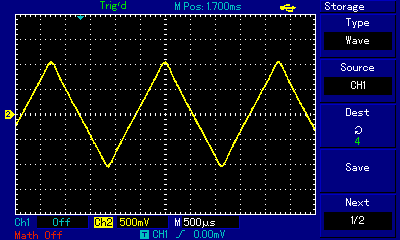
\includegraphics[width=0.9\textwidth]{Synthese_Dreieck.png}
	\caption{Annäherung an ein Dreiecksignal}
	\label{Synthese_Dreieck}
\end{figure}


\begin{figure}[h!]
	\centering
	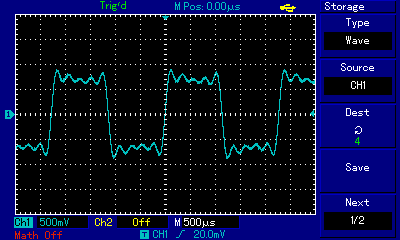
\includegraphics[width=0.9\textwidth]{Synthese_Rechteck.png}
	\caption{Annäherung an ein Rechtecksignal}
	\label{Synthese_Rechteck}
\end{figure}


\begin{figure}[h!]
	\centering
	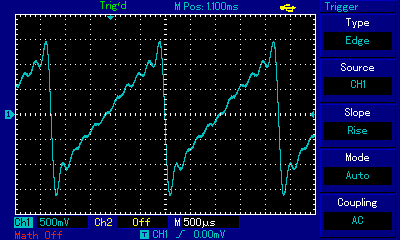
\includegraphics[width=0.9\textwidth]{Synthese_Saegezahn.png}
	\caption{Annäherung an ein Sägezahnsignal}
	\label{Synthese_Saege}
\end{figure}






\clearpage
\subsection{Fourieranalyse}
Für die Auswertung Dreieck-, Rechteck-, und Sägezahnsignal werden die Fourierkoeffizienten eines eingespeisten Signals analysiert. In Unterkapiteln für jedes einzelne Signal befinden sich die Abbildungen, die am Oszilloskop zu sehen sind (Abbildung \ref{Frequenz_Dreieck}, \ref{Frequenz_Rechteck}, \ref{Frequenz_Saege}), Tabellen mit den abgelesenen und ausgerechneten Fourierkoeffizienten (Tabelle: \ref{tab:Dreieck}, \ref{tab:Rechteck}, \ref{tab:Saege})  und eine Visualsierung selbiger (Abbildung: \ref{Fourier_Dreieck}, \ref{Fourier_Rechteck}, \ref{Fourier_Saege}).
Die przentuale Abweichung $\delta a$ der einzelnen gemessenen Koeffizienten $a_\text{gem.}$ von den errechneten $a_\text{ber.}$ ergibt sich nach
\begin{equation}
\delta a = \left(1 - \frac{a_\text{gem.}}{a_\text{ber.}}\right) \cdot 100 \%
\end{equation}
Die eingezeichneten Fehlerbalken beziehen sich auf die Gesamtabweichung von der erwarteten Funktion. Mehr dazu folgt in der Diskussion (Kapitel  \ref{sec:Diskussion}).
Sie wurden hier wie folgt berechnet
\begin{equation}
\Delta a =\sqrt{ \frac{1}{N-2} \sum_{i=2}^{N} (a_\text{gem.} - a_\text{ber.})^2 } \ .
\label{eq:Abweichung}
\end{equation}
Es ist wichtig, bei dem zweiten Wert zu beginnen, da der erste keine Abweichung haben kann. Deswegen wir auch durch $N-2$ geteilt, statt durch $N-1$.
\clearpage

\subsubsection{Dreiecksignal - Fourieranalyse}

\begin{figure}[h!]
	\centering
	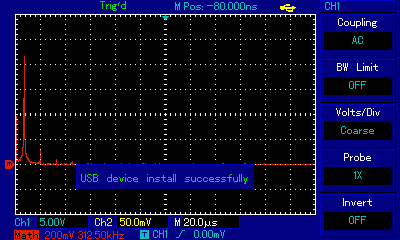
\includegraphics[width=0.6\textwidth]{Dreieck.png}
	\caption{Frequenzspektrum Dreiecksignal}
	\label{Frequenz_Dreieck}
\end{figure}

\begin{figure}[h!]
	\centering
	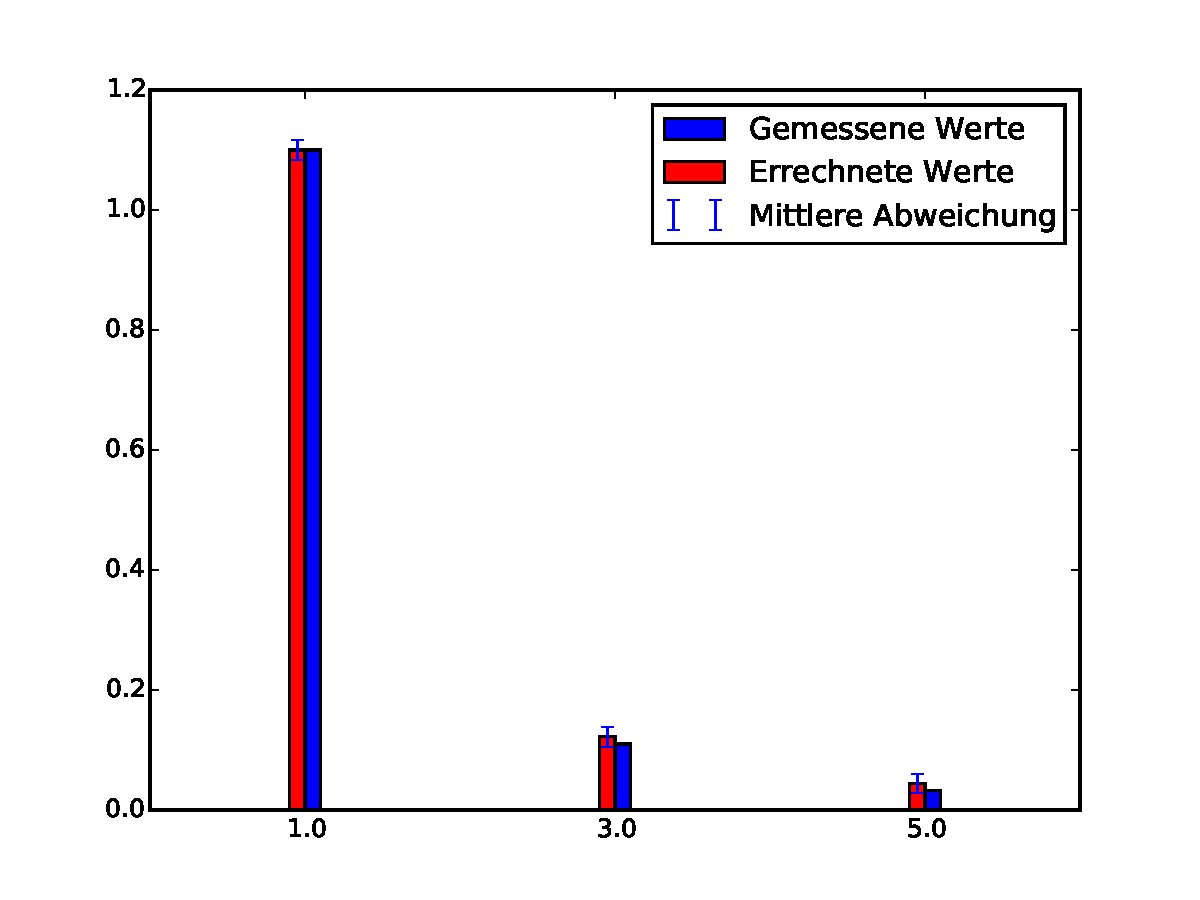
\includegraphics[width=0.6\textwidth]{Dreieck_Fourier.pdf}
	\caption{Frequenzspektrum Dreiecksignal}
	\label{Fourier_Dreieck}
\end{figure}

\begin{figure}[h!]
	\centering
	\captionof{table}{Fourier-Koeffizienten}
	\begin{tabular}{c|ccr}
		& gemessen in V & berechnet in V & Abweichung \\
		\hline
		k =	1 & 1.100   & 1.100      &  0 \%       \\
		k =	3 & 0.110  & 0.122 & -11 \% \\
		k =	5 & 0.033 & 0.044    & -33 \% \\
	\end{tabular}
	\label{tab:Dreieck}
\end{figure}
\clearpage



\subsubsection{Rechtecksignal - Fourieranalyse}


\begin{figure}[h!]
	\centering
	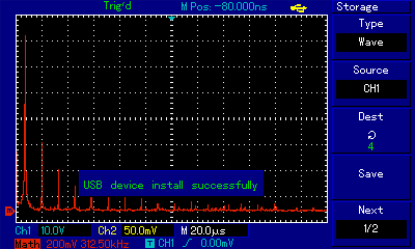
\includegraphics[width=0.6\textwidth]{Rechteck.png}
	\caption{Frequenzspektrum Rechtecksignal}
	\label{Frequenz_Rechteck}
\end{figure}

\begin{figure}[h!]
	\centering
	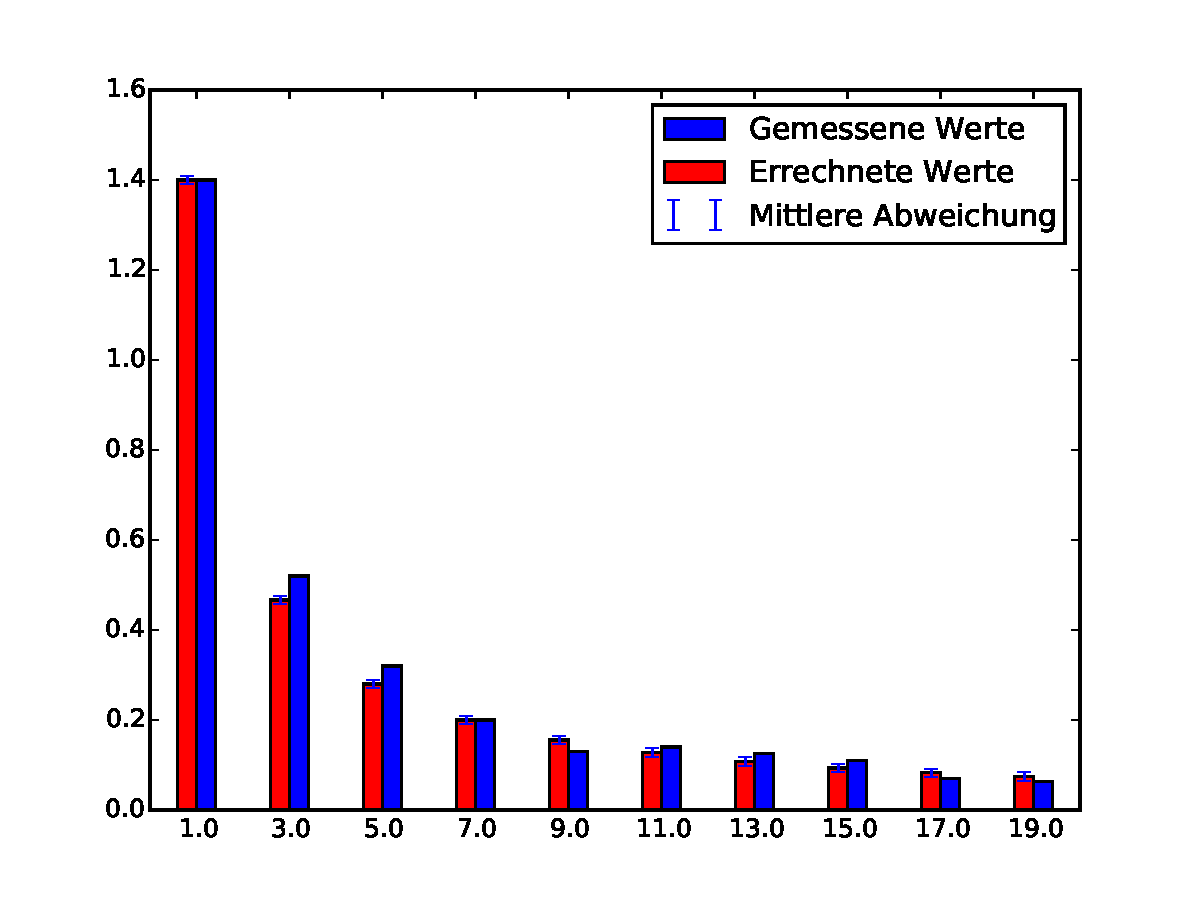
\includegraphics[width=0.6\textwidth]{Rechteck_Fourier.pdf}
	\caption{Frequenzspektrum Rechtecksignal}
	\label{Fourier_Rechteck}
\end{figure}

\begin{figure}[h!]
	\centering
	\captionof{table}{Fourier-Koeffizienten}
	\begin{tabular}{c|ccr}
		& gemessen in V & berechnet in V & Abweichung \\
		\hline
		k = 1 & 1.400   & 1.400       &  0   \%      \\
		k = 3 & 0.520  & 0.467 &  10.3 \%  \\
		k = 5 & 0.320  & 0.280      &  12.5  \%    \\
		k = 7 & 0.200   & 0.200       &  0  \%        \\
		k = 9 & 0.130  & 0.156  & -19.7 \%  \\
		k = 11 & 0.140  & 0.127  &  9.10 \% \\
		k = 13 & 0.125 & 0.108  &  13.8 \%  \\
		k = 15 & 0.110  & 0.093 &  15.2 \% \\
		k = 17 & 0.070  & 0.082 & -17.6 \%  \\
		k = 19 & 0.063 & 0.074 & -17.0 \% \\
	\end{tabular}
	\label{tab:Rechteck}
\end{figure}




\subsubsection{Sägezahnsignal - Fourieranalyse}
\begin{figure}[h!]
	\centering
	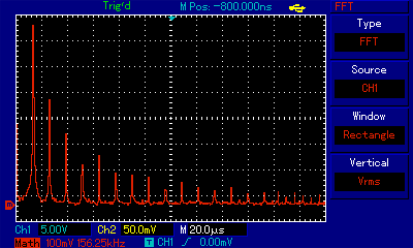
\includegraphics[width=0.6\textwidth]{Saegezahn.png}
	\caption{Frequenzspektrum Sägezahnsignal}
	\label{Frequenz_Saege}
\end{figure}

\begin{figure}[h!]
	\centering
	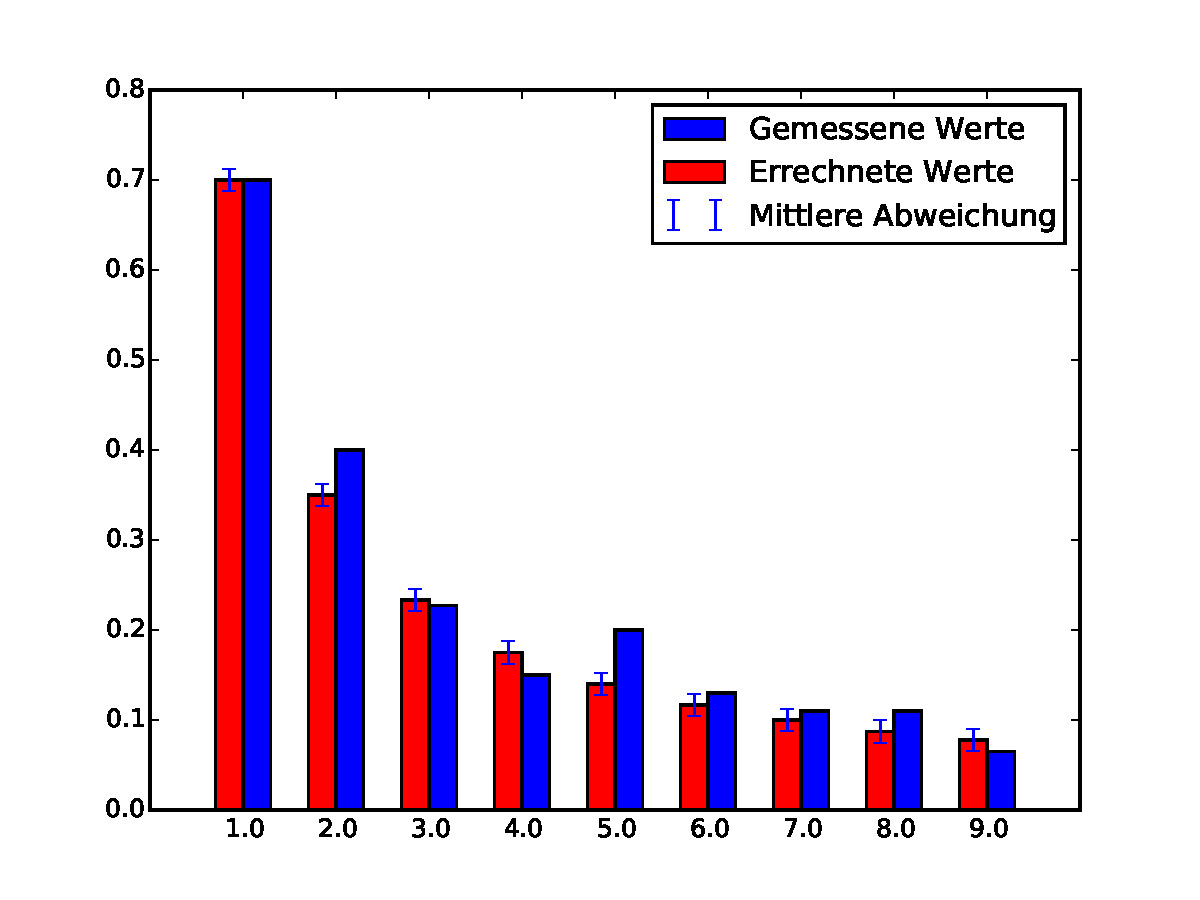
\includegraphics[width=0.6\textwidth]{Saegezahn_Fourier.pdf}
	\caption{Frequenzspektrum Sägezahnsignal}
	\label{Fourier_Saege}
\end{figure}

\begin{figure}[h!]
	\centering
	\captionof{table}{Fourier-Koeffizienten}
	\begin{tabular}{c|ccr}
		& gemessen in V & berechnet in V & Abweichung \\
		\hline
		 k = 1 & 0.700   & 0.700       &  0  \%       \\
		 k = 2 & 0.400   & 0.350      &  12.5 \%     \\
		 k = 3 & 0.227 & 0.233  & -02.8 \% \\
		 k = 4 & 0.150  & 0.175     & -16.7 \%  \\
		 k = 5 & 0.200   & 0.140      &  30.0 \%      \\
		 k = 6 & 0.130  & 0.117  &  10.3 \%  \\
		 k = 7 & 0.110  & 0.100       &  9.10 \% \\
		 k = 8 & 0.110  & 0.086    &  20.5 \%  \\
		 k = 9 & 0.065 & 0.078 & -19.7 \%  \\
	\end{tabular}
	\label{tab:Saege}
\end{figure}
\clearpage

\clearpage


\section{Diskussion}
Ablesefehler
Warmeverluste beim warten
Messfehler bei den Temperaturen der Korper (Korper wird rausgeholt, kuhlt schon aus, wahrend das Thermometer noch steigt)
Atomwarme pro Mol bei Graphit bei konstantem Volumen 161.954
Atomwarme pro Mol bei Blei bei konstantem Volumen 106.5 +-  5.0
Atomwarme pro Mol nach Dulon-Petit 24.573


\clearpage
\listoftodos
\listoffigures
\listoftables
\clearpage
\nocite{\V}
\printbibliography[title = Literaturverzeichnis]

\end{document}
